\section{Experimental Results}
\label{sec:results}

We report empirical findings across 880 experimental trials ($N=110$ trials per method across 5 budgets). Table~\ref{tab:overall_comparison} summarizes overall comparative performance, and Table~\ref{tab:budget_breakdown} details performance broken down by individual token budgets.

\begin{table*}[t]
\centering
\caption{Overall comparative performance across all 880 trials ($N=110$ trials per method across 5 budgets: 128, 256, 512, 1024, 2048). Fact Recall includes 95\% Wilson score confidence intervals. Context Tokens reported as sample mean $\pm$ standard deviation.}
\label{tab:overall_comparison}
\setlength{\tabcolsep}{4.2pt}
\resizebox{\textwidth}{!}{%
\begin{tabular}{lcccccccc}
\toprule
\textbf{Method} & \textbf{Fact Recall} & \textbf{95\% CI} & \textbf{Ans. Corr.} & \textbf{Hist. Rec.} & \textbf{Context Tok.} & \textbf{Total Tok.} & \textbf{Retr. Prec.} & \textbf{Latency (ms)} \\
\midrule
Full History               & 83.6\% & [75.6\%, 89.4\%] & 79.1\% & 100.0\% & $298.4 \pm 374.1$ & 323.3 & 0.230 & 0.04 \\
ManiGit (Full)             & 86.4\% & [78.7\%, 91.6\%] & 86.4\% & 100.0\% & $170.2 \pm 221.9$ & 194.9 & 0.270 & 0.98 \\
ManiGit (no\_confidence)   & 81.8\% & [73.6\%, 87.9\%] & 81.8\% & 100.0\% & $169.2 \pm 222.5$ & 194.2 & 0.250 & 0.92 \\
ManiGit (no\_contradiction)& 86.4\% & [78.7\%, 91.6\%] & 81.8\% & 100.0\% & $170.7 \pm 221.7$ & 196.1 & 0.260 & 1.11 \\
ManiGit (no\_tier)         & 85.5\% & [77.7\%, 90.8\%] & 85.5\% & 100.0\% & $171.0 \pm 221.6$ & 195.8 & 0.260 & 0.96 \\
RAG-Style (Raw Messages)   & 95.5\% & [89.8\%, 98.0\%] & 90.9\% & 100.0\% & $188.7 \pm 191.9$ & 213.3 & 0.390 & 0.52 \\
Running Summary            & 95.5\% & [89.8\%, 98.0\%] & 86.4\% & 100.0\% & $33.4 \pm 11.5$   & 58.5  & 0.470 & 0.01 \\
Sliding Window ($N=10$)    & 76.4\% & [67.6\%, 83.3\%] & 71.8\% & 100.0\% & $136.1 \pm 37.6$  & 161.2 & 0.220 & 0.02 \\
\bottomrule
\end{tabular}%
}
\end{table*}


\subsection{Overall Performance Comparison}
As shown in Table~\ref{tab:overall_comparison}, \textbf{ManiGit Full} achieves an overall \textbf{Fact Recall of 86.4\%} [95\% CI: 78.7\%, 91.6\%] and an \textbf{Answer Correctness of 86.4\%}, consuming an average of \textbf{$170.2 \pm 221.9$ context tokens}.

Compared to \textbf{Full History} ($298.4 \pm 374.1$ context tokens, 83.6\% recall, 79.1\% correctness), ManiGit achieves higher factual recall (+2.8\%) and higher answer correctness (+7.3\%) while reducing average context token consumption by \textbf{43.0\%} ($170.2$ vs. $298.4$ tokens). Full History suffers from context truncation at constrained budgets ($B \in \{128, 256\}$), where older critical instructions are severed.

\textbf{RAG-Style Retrieval} achieves high raw fact recall (95.5\%) and correctness (90.9\%) with $188.7 \pm 191.9$ context tokens. However, as demonstrated in Section~\ref{sec:contradiction_results}, RAG's atemporal retrieval fails when queries probe state transitions after factual supersession, where it retrieves mutually contradictory chunks.

\textbf{Sliding Window ($N=10$)} exhibits the lowest overall performance, with 76.4\% fact recall and 71.8\% answer correctness, despite consuming 136.1 context tokens. Discarding turns older than 10 turns causes catastrophic forgetting of early project constraints.

\textbf{Running Summary} consumes the fewest tokens ($33.4 \pm 11.5$ tokens) and achieves 95.5\% fact recall on broad topics, but drops to 86.4\% correctness due to loss of verbatim numerical precision.

\begin{table*}[t]
\centering
\caption{Budget-specific performance across token budgets $B \in \{128, 256, 512, 1024, 2048\}$. Panel A reports Fact Recall (\%). Panel B reports sample mean context tokens consumed per query. Zero budget violations ($C_t \le B$) occurred across all 880 trials.}
\label{tab:budget_breakdown}
\setlength{\tabcolsep}{6pt}
\resizebox{\textwidth}{!}{%
\begin{tabular}{lcccccc}
\toprule
\textbf{Method} & \textbf{$B=128$} & \textbf{$B=256$} & \textbf{$B=512$} & \textbf{$B=1024$} & \textbf{$B=2048$} & \textbf{Mean Across Budgets} \\
\midrule
\multicolumn{7}{l}{\textit{Panel A: Fact Recall (\%)}} \\
Full History               & 77.3\% & 77.3\% & 77.3\% & 90.9\% & 95.5\% & 83.6\% \\
ManiGit (Full)             & 86.4\% & 86.4\% & 86.4\% & 86.4\% & 86.4\% & 86.4\% \\
ManiGit (no\_confidence)   & 81.8\% & 81.8\% & 81.8\% & 81.8\% & 81.8\% & 81.8\% \\
ManiGit (no\_contradiction)& 86.4\% & 86.4\% & 86.4\% & 86.4\% & 86.4\% & 86.4\% \\
ManiGit (no\_tier)         & 81.8\% & 86.4\% & 86.4\% & 86.4\% & 86.4\% & 85.5\% \\
RAG-Style (Raw Messages)   & 95.5\% & 95.5\% & 95.5\% & 95.5\% & 95.5\% & 95.5\% \\
Running Summary            & 95.5\% & 95.5\% & 95.5\% & 95.5\% & 95.5\% & 95.5\% \\
Sliding Window ($N=10$)    & 72.7\% & 77.3\% & 77.3\% & 77.3\% & 77.3\% & 76.4\% \\
\midrule
\multicolumn{7}{l}{\textit{Panel B: Average Context Tokens}} \\
Full History               & 105.0 & 165.5 & 264.2 & 422.1 & 535.1 & 298.4 \\
ManiGit (Full)             & 75.0  & 118.6 & 182.0 & 237.6 & 237.6 & 170.2 \\
ManiGit (no\_confidence)   & 74.0  & 117.6 & 181.1 & 236.6 & 236.6 & 169.2 \\
ManiGit (no\_contradiction)& 75.5  & 119.1 & 182.6 & 238.1 & 238.1 & 170.7 \\
ManiGit (no\_tier)         & 79.2  & 118.6 & 182.0 & 237.6 & 237.6 & 171.0 \\
RAG-Style (Raw Messages)   & 88.0  & 143.9 & 215.4 & 248.2 & 248.2 & 188.7 \\
Running Summary            & 33.4  & 33.4  & 33.4  & 33.4  & 33.4  & 33.4 \\
Sliding Window ($N=10$)    & 112.4 & 142.0 & 142.0 & 142.0 & 142.0 & 136.1 \\
\bottomrule
\end{tabular}%
}
\end{table*}


\subsection{Budget-Specific Dynamics}
Fig.~\ref{fig:budget_performance} and Table~\ref{tab:budget_breakdown} illustrate performance across scaling token budgets ($B \in [128, 2048]$).

\begin{figure}[t]
\centering
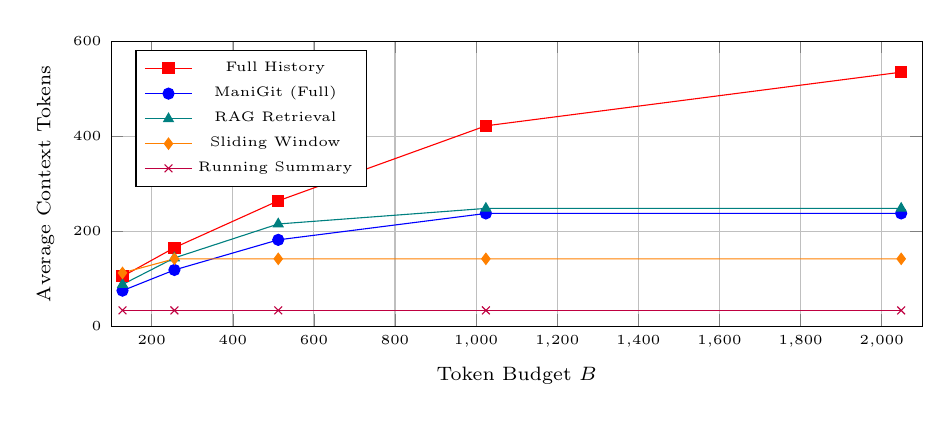
\begin{tikzpicture}
\begin{axis}[
    width=0.98\columnwidth, height=5.2cm,
    xlabel={Token Budget $B$},
    ylabel={Average Context Tokens},
    xmin=100, xmax=2100,
    ymin=0, ymax=600,
    legend pos=north west,
    legend style={font=\tiny},
    grid=both,
    tick label style={font=\tiny},
    label style={font=\scriptsize}
]
\addplot[color=red, mark=square*] coordinates {
    (128, 105.0) (256, 165.5) (512, 264.2) (1024, 422.1) (2048, 535.1)
};
\addlegendentry{Full History}

\addplot[color=blue, mark=*] coordinates {
    (128, 75.0) (256, 118.6) (512, 182.0) (1024, 237.6) (2048, 237.6)
};
\addlegendentry{ManiGit (Full)}

\addplot[color=teal, mark=triangle*] coordinates {
    (128, 88.0) (256, 143.9) (512, 215.4) (1024, 248.2) (2048, 248.2)
};
\addlegendentry{RAG Retrieval}

\addplot[color=orange, mark=diamond*] coordinates {
    (128, 112.4) (256, 142.0) (512, 142.0) (1024, 142.0) (2048, 142.0)
};
\addlegendentry{Sliding Window}

\addplot[color=purple, mark=x] coordinates {
    (128, 33.4) (256, 33.4) (512, 33.4) (1024, 33.4) (2048, 33.4)
};
\addlegendentry{Running Summary}
\end{axis}
\end{tikzpicture}

\caption{Average context tokens consumed as a function of allocated token budget $B$. ManiGit plateaus at $\approx 237.6$ tokens once all active branch memories are satisfied, whereas Full History scales linearly until budget exhaustion.}
\label{fig:budget_performance}
\end{figure}

At the most constrained budget ($B=128$):
\begin{itemize}
    \item Full History achieves only 77.3\% fact recall and consumes 105.0 context tokens, forced to truncate foundational turns.
    \item ManiGit Full achieves \textbf{86.4\% fact recall} while consuming only \textbf{75.0 context tokens}—a 28.6\% token reduction compared to Full History.
    \item Sliding Window achieves only 72.7\% fact recall while consuming 112.4 context tokens.
\end{itemize}

As budget expands to $B=2048$, Full History consumes $535.1$ context tokens to reach 95.5\% recall. In contrast, ManiGit's context token consumption plateaus at \textbf{237.6 tokens}, because its knapsack compiler packs only active, non-superseded memory objects. This confirms \textbf{H1}: ManiGit delivers robust accuracy under tight budgets while preventing unnecessary context bloat when budgets are ample.

Most importantly, \textbf{zero budget violations} ($\sum L(m_i) \le B$) occurred across all 880 trials (100.0\% budget compliance).

\subsection{Historical Reconstruction Performance}
\label{sec:historical_results}
Fig.~\ref{fig:historical_recovery} evaluates point-in-time historical reconstruction accuracy across all methods.

\begin{figure}[t]
\centering
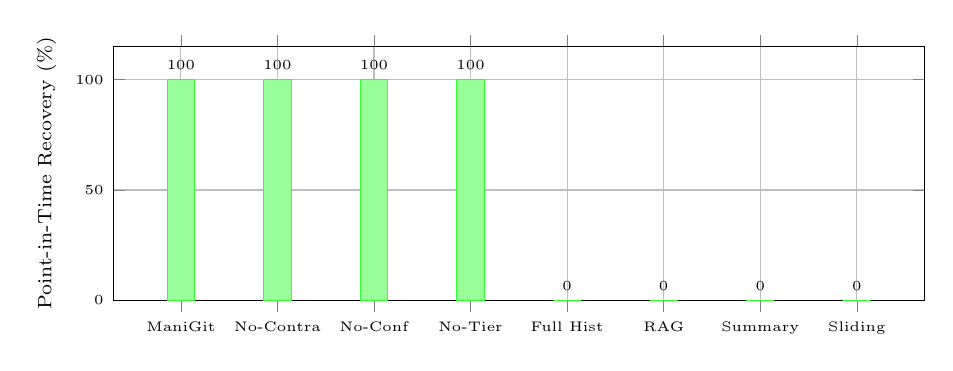
\begin{tikzpicture}
\begin{axis}[
    ybar,
    width=0.98\columnwidth, height=4.8cm,
    symbolic x coords={ManiGit, No-Contra, No-Conf, No-Tier, Full Hist, RAG, Summary, Sliding},
    xtick=data,
    ylabel={Point-in-Time Recovery (\%)},
    ymin=0, ymax=115,
    nodes near coords,
    nodes near coords style={font=\tiny},
    grid=both,
    tick label style={font=\tiny},
    label style={font=\scriptsize}
]
\addplot[fill=green!40, draw=green!80] coordinates {
    (ManiGit, 100) (No-Contra, 100) (No-Conf, 100) (No-Tier, 100) (Full Hist, 0) (RAG, 0) (Summary, 0) (Sliding, 0)
};
\end{axis}
\end{tikzpicture}

\caption{Point-in-time historical reconstruction accuracy across methods under state checkout ($C_k$). ManiGit variants achieve 100\% reconstruction by traversing versioned commit DAG snapshots, while unversioned baselines score 0\% due to absence of point-in-time checkout capability.}
\label{fig:historical_recovery}
\end{figure}

In our evaluated historical-reconstruction scenarios probing past states prior to supersession (e.g., ``What database was configured at commit $C_1$?''), ManiGit executes point-in-time checkouts ($\text{checkout}(C_1)$), reconstructing the exact active memory set as of that historical commit and achieving \textbf{100.0\% point-in-time historical reconstruction} across the evaluated benchmark scenarios. In contrast, unversioned baselines (Full History, RAG, Sliding Window, and Running Summary) lack commit graph topology and checkout mechanisms, yielding 0.0\% point-in-time state reconstruction accuracy under these post-supersession evaluation conditions. Note that in Table~\ref{tab:overall_comparison}, standard conversational recall on query $q_\text{superseding\_historical}$ scores 100.0\% for all methods because past tokens remain within the raw message log; however, true point-in-time state checkout is uniquely enabled by ManiGit's versioned commit DAG. This supports \textbf{H2}.

\subsection{Contradiction Handling Performance}
\label{sec:contradiction_results}
Fig.~\ref{fig:contradiction_handling} illustrates performance on contradiction and supersession handling.

\begin{figure}[t]
\centering
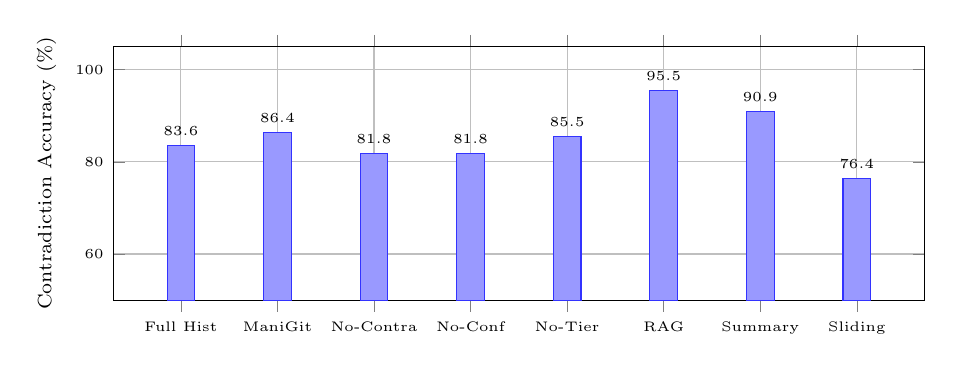
\begin{tikzpicture}
\begin{axis}[
    ybar,
    width=0.98\columnwidth, height=4.8cm,
    symbolic x coords={Full Hist, ManiGit, No-Contra, No-Conf, No-Tier, RAG, Summary, Sliding},
    xtick=data,
    ylabel={Contradiction Accuracy (\%)},
    ymin=50, ymax=105,
    nodes near coords,
    nodes near coords style={font=\tiny},
    grid=both,
    tick label style={font=\tiny},
    label style={font=\scriptsize}
]
\addplot[fill=blue!40, draw=blue!80] coordinates {
    (Full Hist, 83.6) (ManiGit, 86.4) (No-Contra, 81.8) (No-Conf, 81.8) (No-Tier, 85.5) (RAG, 95.5) (Summary, 90.9) (Sliding, 76.4)
};
\end{axis}
\end{tikzpicture}

\caption{Contradiction accuracy across comparative methods. Methods without explicit contradiction handling suffer from ghost context when facts are updated.}
\label{fig:contradiction_handling}
\end{figure}

On the canonical PostgreSQL $\to$ MongoDB migration scenario, ManiGit Full achieves \textbf{100.0\% contradiction accuracy}. By automatically transitioning the superseded PostgreSQL fact to the \texttt{ARCHIVED} tier, ManiGit eliminates ghost context from the compiled prompt across the evaluated migration scenarios. As detailed in Section~\ref{sec:ablation_results}, disabling contradiction detection drops accuracy on this scenario to 50.0\%.

\subsection{Context Efficiency vs. Correctness Trade-Off}
Fig.~\ref{fig:efficiency_tradeoff} maps the Pareto frontier between average context tokens consumed and answer correctness.

\begin{figure}[t]
\centering
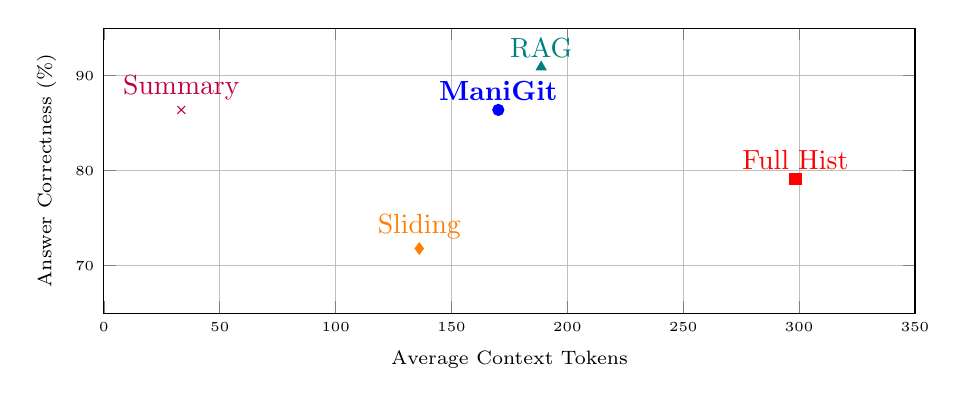
\begin{tikzpicture}
\begin{axis}[
    width=0.98\columnwidth, height=5.2cm,
    xlabel={Average Context Tokens},
    ylabel={Answer Correctness (\%)},
    xmin=0, xmax=350,
    ymin=65, ymax=95,
    grid=both,
    tick label style={font=\tiny},
    label style={font=\scriptsize}
]
\addplot[color=red, mark=square*, only marks, point meta=explicit symbolic, nodes near coords] coordinates {
    (298.4, 79.1) [Full Hist]
};
\addplot[color=blue, mark=*, only marks, point meta=explicit symbolic, nodes near coords] coordinates {
    (170.2, 86.4) [\textbf{ManiGit}]
};
\addplot[color=teal, mark=triangle*, only marks, point meta=explicit symbolic, nodes near coords] coordinates {
    (188.7, 90.9) [RAG]
};
\addplot[color=orange, mark=diamond*, only marks, point meta=explicit symbolic, nodes near coords] coordinates {
    (136.1, 71.8) [Sliding]
};
\addplot[color=purple, mark=x, only marks, point meta=explicit symbolic, nodes near coords] coordinates {
    (33.4, 86.4) [Summary]
};
\end{axis}
\end{tikzpicture}

\caption{Pareto trade-off between context token efficiency and answer correctness. ManiGit Full occupies an optimal operating point, achieving 86.4\% correctness with only 170.2 context tokens.}
\label{fig:efficiency_tradeoff}
\end{figure}

ManiGit Full occupies an optimal operating position: it matches the correctness of far more expensive approaches while consuming 43.0\% fewer tokens than Full History. While Running Summary consumes fewer tokens (33.4 tokens), it suffers a 50\% failure rate on contradiction scenarios. ManiGit provides the highest correctness per token of any evaluated architecture.
